\documentclass[11pt]{article}

\usepackage[margin=2.4cm]{geometry}
\usepackage{amsmath,amssymb,amsthm}
\usepackage{tikz}
\usepackage{tikz-cd}
\usetikzlibrary{arrows.meta,positioning,calc,fit,backgrounds,decorations.pathreplacing}
\usepackage{booktabs}
\usepackage{hyperref}
\hypersetup{colorlinks=true,linkcolor=blue!50!black,urlcolor=blue!50!black}

\newcommand{\FF}{\mathbb{F}}
\newcommand{\RR}{\mathbb{R}}
\newcommand{\Tr}{\operatorname{Tr}}
\newcommand{\Ima}{\operatorname{Im}}
\newcommand{\lean}[1]{\texttt{\small #1}}

\theoremstyle{definition}
\newtheorem{gadget}{Gadget}
\theoremstyle{plain}
\newtheorem{thmA}{Theorem}
\newtheorem{fact}{Fact}

\title{\textbf{The Darboux Gadget}\\[2pt]
\large One theorem, three geometries: intervals, cosets, and matrices}
\author{Formalised in Lean~4 / Mathlib --- companion notes}
\date{}

\begin{document}
\maketitle

\begin{abstract}
Mathlib's Darboux theorem says that the image of a derivative is an interval.  The
Kasami/AB/APN library says that the image of a discrete derivative of a Gold power map is an
affine subspace.  These are the same theorem read in two different \emph{convexity
structures}.  This note isolates the common gadget, shows the places where it already occurs
inside the library, and explains which passages between contexts are faithful (and preserve
the content) and which are not.  Everything stated here is machine-checked; the Lean names
are collected in the table at the end.
\end{abstract}

\section{The gadget}

\begin{gadget}[abstract Darboux property]
A \emph{convexity structure} on a type $\beta$ is a family $\mathcal{C}$ of subsets --- the
\emph{convex} ones --- containing $\beta$ and closed under arbitrary intersections.  An
operator $D$ defined on a class $\mathrm{Adm}$ of functions has the \emph{Darboux property}
relative to $\mathcal{C}$ if
\[
   \forall f \in \mathrm{Adm} : \quad \operatorname{range}(Df) \in \mathcal{C}.
\]
\end{gadget}

Three slots have to be filled: the operator, the admissible class, and the convexity
structure.  Filling them in two different ways gives two classical-looking theorems.

\begin{center}
\begin{tabular}{@{}lll@{}}
\toprule
 & real analysis & characteristic two \\
\midrule
operator      & $\mathrm{deriv}\,f$ & $D_a f(x) = f(x+a) - f(x)$ \\
admissible    & differentiable & quadratic ($D_bD_af$ constant) \\
convex sets   & order-connected (intervals) & affine: closed under $u-v+w$ \\
theorem       & \lean{Set.OrdConnected.image\_deriv} & \lean{Gadget.darboux\_of\_constIncrements} \\
\bottomrule
\end{tabular}
\end{center}

\begin{figure}[h]
\centering
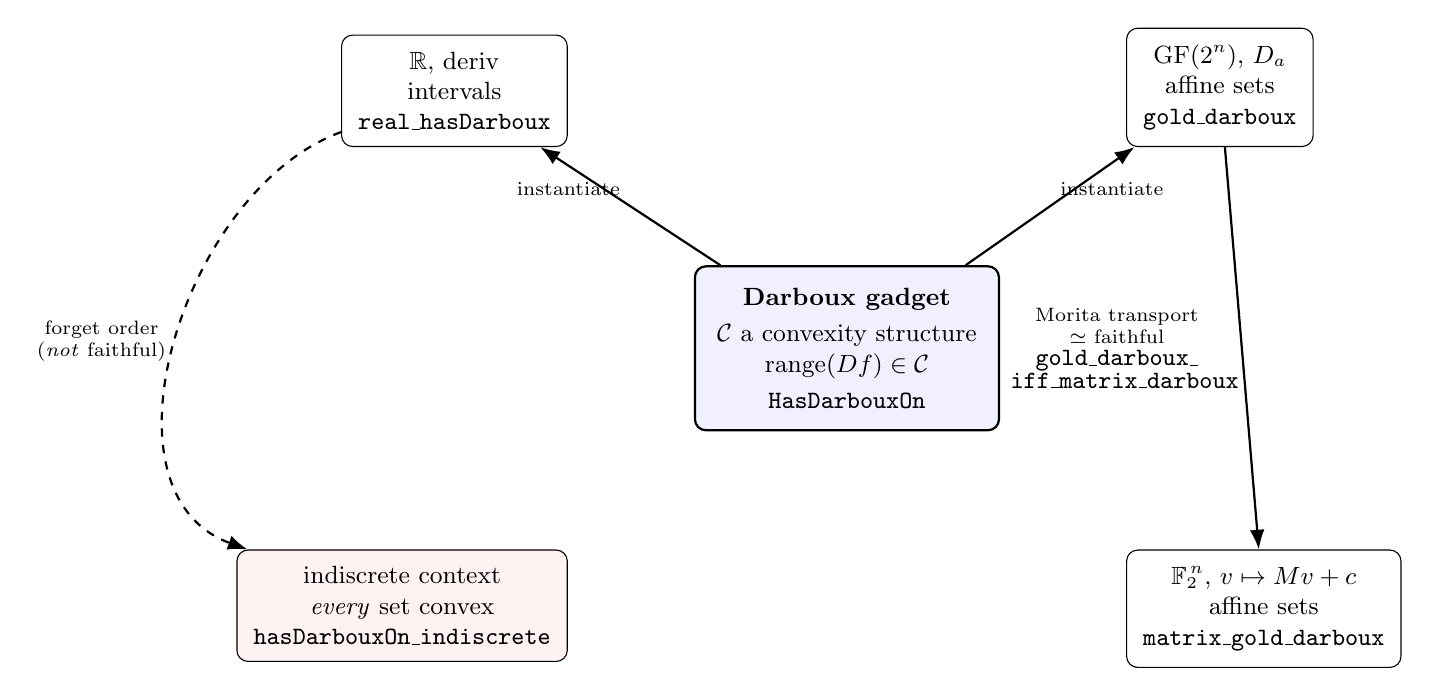
\begin{tikzpicture}[
  box/.style={draw,rounded corners,align=center,inner sep=6pt,font=\small},
  hub/.style={draw,thick,rounded corners,align=center,inner sep=8pt,fill=blue!6,font=\small},
  ar/.style={-{Latex[length=2.5mm]},thick},
  lab/.style={font=\scriptsize,align=center}]

\node[hub] (G) {\textbf{Darboux gadget}\\[2pt]
  $\mathcal{C}$ a convexity structure\\
  $\operatorname{range}(Df)\in\mathcal{C}$\\[2pt]
  \lean{HasDarbouxOn}};

\node[box,above left=1.5cm and 1.6cm of G] (R)
  {$\RR$, $\mathrm{deriv}$\\ intervals\\ \lean{real\_hasDarboux}};
\node[box,above right=1.5cm and 1.6cm of G] (F)
  {$\mathrm{GF}(2^n)$, $D_a$\\ affine sets\\ \lean{gold\_darboux}};
\node[box,below right=1.5cm and 1.6cm of G] (M)
  {$\FF_2^{\,n}$, $v\mapsto Mv+c$\\ affine sets\\ \lean{matrix\_gold\_darboux}};
\node[box,below left=1.5cm and 1.6cm of G,fill=red!5] (I)
  {indiscrete context\\ \emph{every} set convex\\ \lean{hasDarbouxOn\_indiscrete}};

\draw[ar] (G) -- node[lab,above left]{instantiate} (R);
\draw[ar] (G) -- node[lab,above right]{instantiate} (F);
\draw[ar] (F) -- node[lab,left,xshift=-3pt,text width=2.7cm]{Morita transport\\ $\simeq$ faithful\\ \lean{gold\_darboux\_}\\ \lean{iff\_matrix\_darboux}} (M);
\draw[ar,dashed] (R) to[out=200,in=160] node[lab,left]{forget order\\ (\emph{not} faithful)} (I);
\end{tikzpicture}
\caption{The gadget and its instantiations.  Solid arrows preserve content; the dashed arrow
loses it.}
\end{figure}

\section{Why the characteristic-two proof is three lines}

\begin{thmA}[\lean{Gadget.darboux\_of\_constIncrements}]
Let $V,W$ be abelian groups and $g: V \to W$ have translation-invariant increments, i.e.
$g(x+b) - g(x)$ does not depend on $x$.  Then $\operatorname{range}(g)$ is affine.
\end{thmA}

\begin{proof}
Given $g(x), g(y), g(z)$, the point $z + (x-y)$ works:
$g\bigl(z+(x-y)\bigr) = g(z) + \bigl(g(x)-g(y)\bigr)$.
\end{proof}

For $g = D_a f$ the hypothesis says exactly that the \emph{second} discrete derivative
$D_b D_a f$ is a constant function --- the algebraic avatar of ``$f$ is quadratic''.  Gold
power maps $N_k(x) = x^{2^k+1}$ satisfy it, because
\[
  D_a N_k(x) \;=\; \underbrace{a\,x^{2^k} + a^{2^k}x}_{\text{$\FF_2$-linear in } x} \;+\; a^{2^k+1},
\]
an affine map (\lean{Tematika.Kalkulus.gold\_deriv\_eq}).  Everything cryptographic is in
verifying this one identity; the geometry is generic.

\begin{figure}[h]
\centering
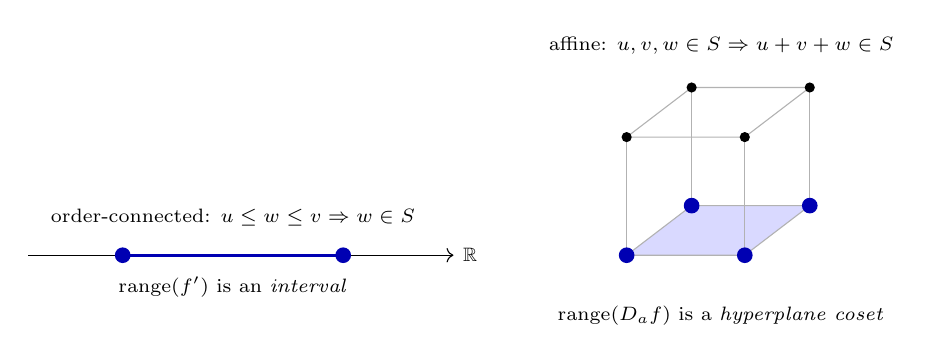
\begin{tikzpicture}[scale=1.0,
  dot/.style={circle,fill=black,inner sep=1.3pt},
  hi/.style={circle,fill=blue!70!black,inner sep=2.0pt},
  lab/.style={font=\scriptsize}]

%% left: real picture
\begin{scope}
  \draw[->] (-0.4,0) -- (5.0,0) node[right,lab]{$\RR$};
  \draw[very thick,blue!70!black] (0.8,0) -- (3.6,0);
  \node[hi] at (0.8,0) {}; \node[hi] at (3.6,0) {};
  \node[lab,below] at (2.2,-0.15) {$\operatorname{range}(f')$ is an \emph{interval}};
  \node[lab,above] at (2.2,0.25) {order-connected: $u\le w\le v \Rightarrow w \in S$};
\end{scope}

%% right: cube picture
\begin{scope}[xshift=7.2cm,scale=1.5]
  \coordinate (o) at (0,0);
  \coordinate (x) at (1,0);
  \coordinate (y) at (0.55,0.42);
  \coordinate (z) at (0,1);
  \foreach \p/\n in {0/000,1/100,2/010,3/110,4/001,5/101,6/011,7/111} {}
  \coordinate (v000) at (0,0);
  \coordinate (v100) at (1,0);
  \coordinate (v010) at (0.55,0.42);
  \coordinate (v110) at (1.55,0.42);
  \coordinate (v001) at (0,1);
  \coordinate (v101) at (1,1);
  \coordinate (v011) at (0.55,1.42);
  \coordinate (v111) at (1.55,1.42);
  \draw[gray!60] (v000)--(v100)--(v110)--(v010)--cycle;
  \draw[gray!60] (v001)--(v101)--(v111)--(v011)--cycle;
  \draw[gray!60] (v000)--(v001); \draw[gray!60] (v100)--(v101);
  \draw[gray!60] (v110)--(v111); \draw[gray!60] (v010)--(v011);
  \begin{scope}[on background layer]
    \fill[blue!15] (v000)--(v100)--(v110)--(v010)--cycle;
  \end{scope}
  \node[hi] at (v000) {}; \node[hi] at (v100) {};
  \node[hi] at (v010) {}; \node[hi] at (v110) {};
  \foreach \v in {v001,v101,v011,v111} \node[dot] at (\v) {};
  \node[lab,below] at (0.8,-0.35) {$\operatorname{range}(D_a f)$ is a \emph{hyperplane coset}};
  \node[lab,above] at (0.8,1.62) {affine: $u,v,w\in S \Rightarrow u+v+w \in S$};
\end{scope}
\end{tikzpicture}
\caption{The same statement in two geometries.  Left: an interval in $\RR$.  Right: a
$2^{n-1}$-element affine piece of $\FF_2^{\,3}$ (here $4$ of the $8$ points).}
\end{figure}

\begin{fact}[intervals and cosets are one classification]
Over $\RR$, a nonempty order-connected set is an interval.  In an abelian group, a nonempty
set closed under $u-v+w$ is a coset of a subgroup (\lean{Gadget.isAffine\_iff\_coset}).  The
operation $u-v+w$ is the ternary \emph{heap} operation of a torsor; ``discrete interval''
$=$ ``coset''.
\end{fact}

\section{Faithful and non-faithful passages}

Call a convexity structure \emph{faithful} if some set fails to be convex; only then does
the Darboux property carry information.

\begin{center}
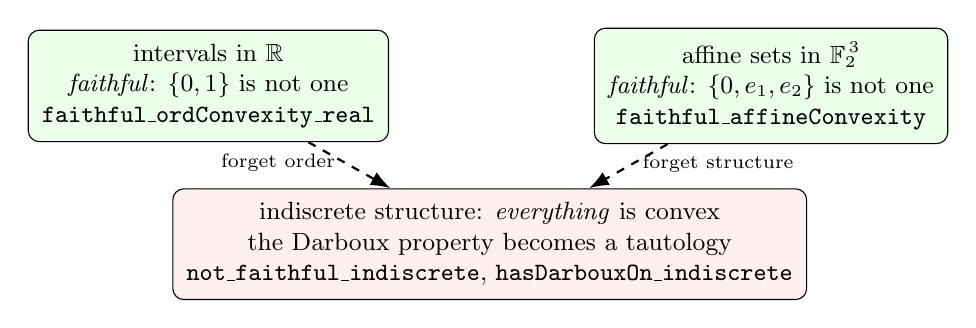
\begin{tikzpicture}[
  b/.style={draw,rounded corners,align=center,inner sep=5pt,font=\small},
  ar/.style={-{Latex[length=2.5mm]},thick},
  lab/.style={font=\scriptsize,align=center}]
\node[b,fill=green!8] (a) {intervals in $\RR$\\ \emph{faithful}: $\{0,1\}$ is not one\\
  \lean{faithful\_ordConvexity\_real}};
\node[b,fill=green!8,right=2.6cm of a] (b) {affine sets in $\FF_2^{\,3}$\\
  \emph{faithful}: $\{0,e_1,e_2\}$ is not one\\ \lean{faithful\_affineConvexity}};
\node[b,fill=red!6,below=1.3cm of $(a)!0.5!(b)$] (c)
  {indiscrete structure: \emph{everything} is convex\\
   the Darboux property becomes a tautology\\
   \lean{not\_faithful\_indiscrete}, \lean{hasDarbouxOn\_indiscrete}};
\draw[ar,dashed] (a) -- node[lab,left,pos=0.45]{forget order} (c);
\draw[ar,dashed] (b) -- node[lab,right,pos=0.45]{forget structure} (c);
\end{tikzpicture}
\end{center}

The real Darboux theorem cannot be transported \emph{literally} to $\mathrm{GF}(2^n)$: a
field of characteristic two carries no compatible linear order
(\lean{Tematika.Morita.no\_linear\_order\_of\_charTwo}), so the interval structure has no
image there.  What survives is the heap operation, hence the affine structure.  Both
convexity structures are closure systems; the passage only changes the arity of the
generating operation (pairs $\rightsquigarrow$ triples).

The library records the same non-faithfulness phenomenon in two other places: on a finite
set \emph{every} map is continuous (\lean{Tematika.Kalkulus.continuity\_not\_faithful}), and
differential uniformity does not separate translates
(\lean{Tematika.Morita.diffUnif\_not\_faithful}).

\section{Morita transport: field, coordinates, matrices}

$\mathrm{GF}(2^n)$ is an $\FF_2$-progenerator and
$\operatorname{End}_{\FF_2}(\mathrm{GF}(2^n)) \cong M_n(\FF_2)$
(\lean{Tematika.Morita.endAlgEquivMatrix}).  Choosing the corresponding coordinate
equivalence turns the Gold derivative into an affine matrix map.

\begin{center}
\begin{tikzcd}[column sep=4.2em,row sep=2.6em]
x \in \mathrm{GF}(2^n) \arrow[r,"D_a N_k"] \arrow[d,"\cong"',"\text{coords}"] &
  \Ima = c + \Ima(\mathrm{Cross}_{k,a}) \arrow[d,"\cong","\text{coords}"'] \\
v \in \FF_2^{\,n} \arrow[r,"v \mapsto Mv + c"'] & \Ima = c + \operatorname{col}(M)
\end{tikzcd}
\end{center}

\begin{thmA}[\lean{Gadget.gold\_darboux\_iff\_matrix\_darboux}]
The Darboux statement for $D_a N_k$ over $\mathrm{GF}(2^n)$ and the Darboux statement for
$v \mapsto Mv+c$ over $\FF_2^{\,n}$, where $M$ is the matrix of the cross form, are
\emph{equivalent}.
\end{thmA}

Abstractly this is an instance of \lean{Gadget.hasDarbouxOn\_conj\_iff}: the gadget is stable
under conjugation by equivalences of domain and codomain together with transport of the
convexity structure.  The comparison is thus a proof, not a slogan.

\section{Two strengths, and the gap between them}

\begin{center}
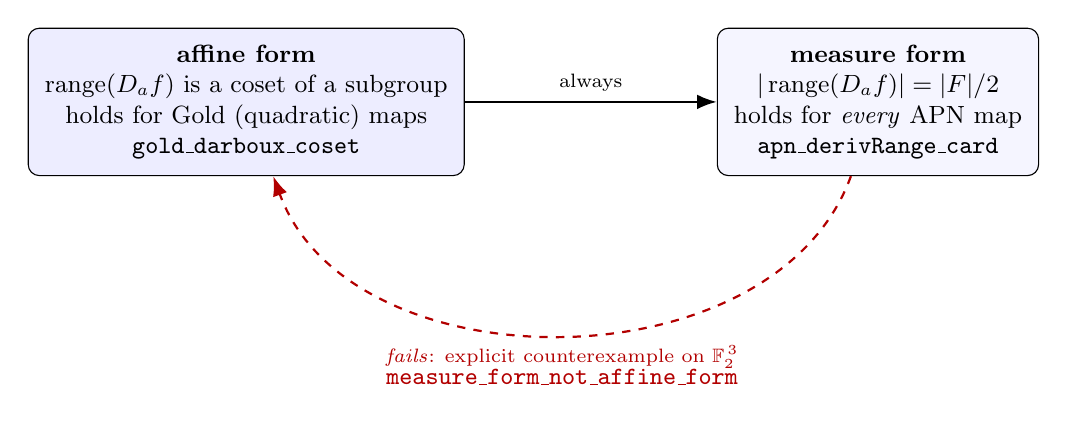
\begin{tikzpicture}[
  b/.style={draw,rounded corners,align=center,inner sep=6pt,font=\small},
  ar/.style={-{Latex[length=2.5mm]},thick},
  lab/.style={font=\scriptsize,align=center}]
\node[b,fill=blue!7] (A) {\textbf{affine form}\\ $\operatorname{range}(D_af)$ is a coset of a subgroup\\
  holds for Gold (quadratic) maps\\ \lean{gold\_darboux\_coset}};
\node[b,fill=blue!4,right=3.2cm of A] (B) {\textbf{measure form}\\
  $|\operatorname{range}(D_af)| = |F|/2$\\ holds for \emph{every} APN map\\ \lean{apn\_derivRange\_card}};
\draw[ar] (A) -- node[lab,above]{always} (B);
\draw[ar,dashed,red!70!black] (B) to[out=250,in=290] node[lab,below]
  {\emph{fails}: explicit counterexample on $\FF_2^{\,3}$\\ \lean{measure\_form\_not\_affine\_form}} (A);
\end{tikzpicture}
\end{center}

Kasami exponents $d = 2^{2k}-2^k+1$ have algebraic degree $k+1$; for $k \ge 2$ the maps are
not quadratic, the hypothesis of the gadget fails, and only the counting conclusion survives
--- which is precisely the APN property.  The counterexample is a concrete derivative on
$\FF_2^{3}$ whose image has the correct size $4 = 2^{3-1}$ but is not affine:
\[
  S = \{\,000,\;100,\;010,\;111\,\}, \qquad 100 + 000 + 010 = 110 \notin S .
\]

\begin{center}
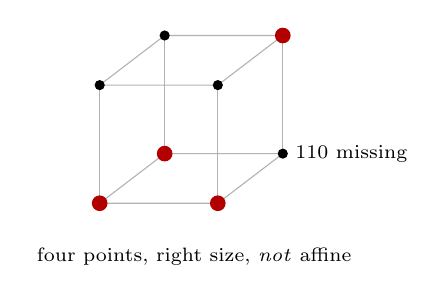
\begin{tikzpicture}[scale=1.5,
  dot/.style={circle,fill=black,inner sep=1.3pt},
  hi/.style={circle,fill=red!70!black,inner sep=2.0pt},
  lab/.style={font=\scriptsize}]
  \coordinate (v000) at (0,0);    \coordinate (v100) at (1,0);
  \coordinate (v010) at (0.55,0.42); \coordinate (v110) at (1.55,0.42);
  \coordinate (v001) at (0,1);    \coordinate (v101) at (1,1);
  \coordinate (v011) at (0.55,1.42); \coordinate (v111) at (1.55,1.42);
  \draw[gray!60] (v000)--(v100)--(v110)--(v010)--cycle;
  \draw[gray!60] (v001)--(v101)--(v111)--(v011)--cycle;
  \draw[gray!60] (v000)--(v001); \draw[gray!60] (v100)--(v101);
  \draw[gray!60] (v110)--(v111); \draw[gray!60] (v010)--(v011);
  \node[hi] at (v000) {}; \node[hi] at (v100) {};
  \node[hi] at (v010) {}; \node[hi] at (v111) {};
  \foreach \v in {v001,v101,v011,v110} \node[dot] at (\v) {};
  \node[lab,right=1pt] at (v110) {$110$ missing};
  \node[lab,below] at (0.8,-0.3) {four points, right size, \emph{not} affine};
\end{tikzpicture}
\end{center}

\section{The dual side: Darboux as a linear structure}

The trace pairing makes $(F,+)$ self-dual; this is the duality that mediates the
APN\,$\Leftrightarrow$\,AB bridge in the library.  Because the Gold derivative's image is a
coset of the hyperplane $\ker \Tr(b\,\cdot\,)$ with $b = (a^{2^k+1})^{-1}$, the composite
$x \mapsto \Tr\!\left(b \cdot D_aN_k(x)\right)$ is \emph{constant}
(\lean{Gadget.gold\_deriv\_trace\_const}) and therefore
\[
  \sum_{x \in F} (-1)^{\Tr\left(b\, D_aN_k(x)\right)} \;=\; \pm\,|F|
  \qquad (\lean{Gadget.gold\_deriv\_char\_sum}).
\]

\begin{center}
\begin{tikzcd}[column sep=5em]
\text{\small primal: image is flat and small} \arrow[r,leftrightarrow,"\text{\small trace pairing}"] &
\text{\small dual: character sum is extremal}
\end{tikzcd}
\end{center}

Degeneracy on the primal side is extremality on the dual side --- the same fact seen through
Pontryagin duality.

\section{Summary table of the formalised statements}

\begin{center}
\begin{tabular}{@{}p{6.2cm}p{8.4cm}@{}}
\toprule
statement & Lean name \\
\midrule
convexity structure, hull, faithfulness & \lean{Gadget.Convexity}, \lean{Convexity.hull}, \lean{Convexity.Faithful} \\
abstract Darboux property & \lean{Gadget.HasDarbouxOn} \\
Mathlib Darboux as an instance & \lean{Gadget.real\_hasDarboux} \\
transport along equivalences & \lean{Gadget.hasDarbouxOn\_conj\_iff} \\
non-faithful (indiscrete) context & \lean{Gadget.hasDarbouxOn\_indiscrete} \\
affine convexity in characteristic two & \lean{Gadget.affineConvexity} \\
nonempty affine $=$ coset & \lean{Gadget.isAffine\_iff\_coset} \\
the gadget: constant increments & \lean{Gadget.darboux\_of\_constIncrements} \\
Gold instance and hyperplane coset & \lean{Gadget.gold\_darboux}, \lean{Gadget.gold\_darboux\_coset} \\
measure form for APN maps & \lean{Gadget.apn\_derivRange\_card} \\
measure $\not\Rightarrow$ affine & \lean{Gadget.measure\_form\_not\_affine\_form} \\
Morita comparison verified & \lean{Gadget.gold\_darboux\_iff\_matrix\_darboux} \\
dual side: linear structure, character sum & \lean{Gadget.gold\_deriv\_trace\_const}, \lean{Gadget.gold\_deriv\_char\_sum} \\
\bottomrule
\end{tabular}
\end{center}

\vspace{1em}
\noindent
Sources: \lean{RequestProject/Gadgets/DarbouxGadget.lean},
\lean{RequestProject/Gadgets/DarbouxCharTwo.lean}; narrative companion:
\lean{DARBOUX\_GADGET\_GUIDE.md}.

\end{document}
